\documentclass[a4paper,12pt]{article} % тип документа

% report, book



%  Русский язык

\usepackage[T2A]{fontenc}			% кодировка
\usepackage[utf8]{inputenc}			% кодировка исходного текста
\usepackage[english,russian]{babel}	% локализация и переносы
\usepackage{graphicx}
\graphicspath{{./}}
\DeclareGraphicsExtensions{.png,.jpg}


% Математика
\usepackage{amsmath,amsfonts,amssymb,amsthm,mathtools} 


\usepackage{wasysym}

%Заговолок
\author{Бредихин Александр}
\title{Домашняя работа №2}
%\date {29 февраля}


\begin{document} % начало документа

\maketitle

\subsection*{Задача 1}
Функция $u(M)$ равна наибольшему числу тактов работы на входных словах длины $10$, если МТ $M$ останавливается на каждом таком слове, и не определена в противном случае. Вычислима ли $u(M)$?\\

Будем доказывать, что функция $u(M)$ -- вычислима. Для этого построим алгоритм, который вычисляет эту функцию:\\
Входные слова длины 10, значит количество входных слов ограничено и равно $ A^{10} $, где $ A $ -- мощность алфавита рассматривваемых МТ (конечное число по определению МТ). Так как входных слов конечное число, то их можно занумеровать. Построим табличку из элементов ($ i , j$), где $j$ - номер входа, $ i $ - номер МТ. Заполняем эту табличку следующим образом: запускаем МТ с номером $i$ на кажжом из входов $j$. Если эта МТ останавливается, то в ячейку ($ i , j$) пишем количество тактов за которое данная МТ остановилась.\\
Функция $u(M)$ - вычислима, так как мы идём по строчке $ M $ описанной выше таблицы:
\begin{itemize}
\item Если МТ останавилась на каждом из входов $ j $, то в каждой ячейке ($ i , j$) написано конечное число. Так как входов конечное число, то затем за один проход по этой строчке можем найти максимум, который и является возвращаемым значением функции (ответ функции получается за конечное время)
\item Если на каком-то из входов $ j $ МТ $ M $ не остановилась, то функция $u(M)$ будет неопределена.
\end{itemize}
Получили алгоритм вычисления $u(M)$, значит она вычислима.\\
Ответ: вычислима.

\subsection*{Задача 3}
Перечислим ли язык $L_\emptyset$ состоящий из всех описаний МТ, которые не останавливаются ни на каком входе? \\

Для начала покажем, что язык $L_\emptyset$ -- коперечеслим, то есть язык $ L^* = L \setminus L_\emptyset $ -- перечеслим (язык всех МТ, которые останавливаются хотя бы на одном входе). Из семинара:\\
$L^* \subset \Sigma^*$ перечислим $\iff$ существует вычислимая функция $R(x, y): \Sigma^*\times\Sigma^* \rightarrow \{0, 1\}$: $x\in L^* \iff \exists y \in \Sigma^*: R(x, y) = 1$.\\ 
Зададим функцию $ R(x,y) $ следующим образом: эта функция запускает МТ $ x $, на входе $ y $: 
если МТ остановилась, то $ R(x,y) = 1 $, иначе $ R(x,y) = 0 $.
Получается:\\
\begin{itemize}
\item если $ x\in L^*  $, то по определению языка $ L^* $ существует хотя бы один вход $ y $, на котором $ x $ остановится, значит $ R(x,y)=1 $\\
\item если $ x\notin L^*  $, следовательно не существует входа $ y $, где $ R(x,y)=1 $\\
\end{itemize}
Значит, язык $ L^* $ - перечеслим. Теперь докажем ещё, что язык $ L^* $ -- неразрешим. Для этого докажем такую сводимость: $ L_{stop} \leq_m L^* $. По определению нужно найти такую вычислимую функцию $ f $, что 
$\left \{\begin{array}{ccc} (M,w) \in L_{stop} & \implies & f([M,w]) \in L^* \\ (M,w) \not \in L_{stop} & \implies & f([M,w]) \not \in L^* \end{array}\right.$\\
Построим служебную МТ: $ M_w $ - которая будет считывать слово $ w $ с ленты, затем возвращать головку МТ в начало слова и завершаться. (Если этой МТ подать слово отличное от $ w $, то она не остановится). Возьмём функцию $ f([M,w])= M_w \circ M  $.
\begin{itemize}
\item Если $ (M,w)\in L_{stop} $ (то есть МТ: $ M $ останавливается на входе $ w $), то $ f([M,w]) $ тоже остановится на входе $ w $, так как МТ $M_w $ передаст выполнение МТ $ M $ на входе $ w $, на котором она останавливается, значит есть хотя бы один вход на котором $ f([M,w]) $ останавливается, следовательно, $ f([M,w]) \in L^*$.
\item Если $ (M,w)\notin L_{stop} $ (то есть МТ: $ M $ не останавливается на входе $ w $), то на входе $ w $ функция $ f([M,w]) $ не остановится. На других входах $ w^* $, функция $ f([M,w]) $ тоже не остановится, так как не останавливается МТ $ M_w $, значит, $ f([M,w]) $ не останавливается на любом входе, значит $ f([M,w]) \notin L^*$
\end{itemize}
Значит $ f $ -- нужная функция и $ L_{stop} \leq_m L^* $. Из семинара язык $ L_{stop} $ не разрешим $ \longrightarrow $ язык $ L^* $ тоже неразрешим.\\
Получается язык $ L^* $ -- перечеслим и неразрешим $ \longrightarrow $ по теореме Поста язык $L_\emptyset = L \setminus L^*$ -- неперечеслим.\\
Ответ: $L_\emptyset$ -- неперечеслим.
 
\subsection*{Задача 2}
Разрешим ли язык $L$, состоящий из всех описаний МТ, у которых есть недостижимое состояние (не достигается ни при каком входе)?\\

\begin{center}
 \textbf{\underline{Замечание}}
\end{center}

Решение использует существование вычислимого алгоритма удаления всех недостижимых состояний, которого, как оказалось после семинара, не существует.\\ По другому не успел решить. Ниже предложено первоначальное решение.\\


Для решения задачи сведём аналогичный язык языку из задачи 3 -- $L_\emptyset$  к данному языку $ L $, то есть покажем, что: $ L_\emptyset \leq_m L $ \\
По определению тогда существует такая вычислимая функция $f$, что\\
 $\left \{\begin{array}{ccc} x \in A & \implies & f(x) \in B \\ x \not \in A & \implies & f(x) \not \in B \end{array}\right.$\\
Возьмём такую функцию $ f $: $ f(M) = M \circ M^\ast $, где $ M^\ast $ - МТ, которая печатает на ленту символ $ \sharp $ и останавливается (все её состояния при работе на любом входе достижимы). А $ M $ - исходная МТ у которой убираются все недостижимые состояния, если такие существуют (функция $ f $ в цикле идёт по таблице переходов МТ (которая конечная) и убирает все состояния в которые нет переходов или в которые есть переход по символу, которого нет а алфавите. Если кол-во состояний перестаёт изменяться, то все недостижимые состояния будут убраны и $ f $ выходит из цикла. Это выполняется за конечное время, значит, функция вычислима). Тогда получается:
\begin{itemize}
\item[1] Если $ M \in L_\emptyset$, то есть не останавливается ни на каком входе, то $ f(M) = M \circ M^\ast $ не остановится на машине $ M $, значит состояния МТ $ M^\ast $ будут недостижимы для $ f(M)$ $ \longrightarrow f(M) \in L $.
\item[2] Если $ M \notin L_\emptyset$, значит существует $ w $(вход), на котором $ M $ остановится, тогда $ f(M) $ на этом входе тоже остановится (так как останавливаются МТ $ M $ и $ M^\ast$) и все состояния $ f(M) $ будут достижимыми (так как у машины $ M $ для каждого состояния существует вход, где это состояние будет достижимо, а теперь ещё будет вход $ w $, где и состояния $ M^\ast$ будут достижимы, значит для какждого состояния $ f(M) $ будет существовать вход, на котором оно будет достижимым, следовательно они все достижимы), то есть $ f(M) \notin L $
\end{itemize}
Получили, что $L_\emptyset \leq_m L$. Язык $L_\emptyset$ - неразрешим (показали в задаче 3), значит данный в этой задаче язык $ L $ тоже неразрешим.\\
Ответ: $ L $ -- неразрешим.




\subsection*{Задача 4}
Показать, что любой перечислимый язык сводится к $L_{stop}$.\\

В предыдущей домашней работе (задаче 2) мы доказали эквивалентность определений: язык $ A $ -- перечеслим $ \Longleftrightarrow $ $ \exists g $ -- вычислимая функция, у которой $ A $ область определения. Значит, существует МТ $ M_g $, которая вычисляет эту функцию, то есть останавливается на словах из $ A $, и не останавливается на других.\\
Построим вспомогательную МТ: $ M_x $, которая печатает на пустой ленте слово x, возвращает головку в начало этого слова и завершается. И возьмём такую функцию $ f(x) = M_x \circ M_g $. \\Тогда:\\
если $ x\in A \longrightarrow f(x) = M_x \circ M_g = L_{stop}(M_g,x) \in L_{stop} $\\
если $ x\notin A \longrightarrow f(x) = M_x \circ M_g \notin L_{stop} $ (так как МТ $ M_x $ не остановится)\\
Следовательно, по определению $m$-сводимости, любой перечислимый язык сводится к $ L_{stop} $

\subsection*{Задача 5}
Верно ли, что все непустые коперечислимые языки $m$-сводятся друг к другу?\\
Ответ: не верно, покажем это:\\
от противного, пусть это утверждение верно.\\
В задаче 3, показали, что непустой язык $L_\emptyset$ коперечеслим и неразрешим. Также язык состоящий из конечного числа элементов -- $A$,  коперечеслим и разрешим\\
Разрешим так как для него можно легко получить характеристическую функцию:
\[
\chi_{W}(x) = \left\{
\begin{array}{cc}
1 & x \in W \\
0 & x \not \in W 
\end{array} \right., 
\]
где $\chi_{W}(x)$ - функция, которая пробегается по всем элементам множества и проверяет, находится ли нужный элемент в нём или нет (так как множество конечно, то такая функция вычислима)\\
Следовательно, язык $A$ и перечеслим.\\
Из теореме Поста:  $A \subset L$ разрешим $\iff A$ и $L \setminus A$ перечислимы $\longrightarrow$ $A$ - коперечеслим.\\
Из нашего предположения эти языки должны $m$-сводятся друг к другу (так как они оба коперечеслимы), то есть 
$L_\emptyset =_m A$
но один из них неразрешим, а другой -- разрешим. Получили противоречие, так как у них должны быть одинаковые свойства: либо оба разрешимы, либо оба неразрешимы, следовательно, все непустые коперечислимые языки \textbf{\textit{не}} $m$-сводятся друг к другу.



\subsection*{Задача 6}
Функция Трудолюбия Радо (busy beaver function) определяется, как максимальное количество единиц, которые может напечатать МТ с $n$ состояниями перед остановкой.\\

{\bf a)} Функция всюду определена, так как количество МТ с $ n $ состояниями -- конечное число. Те которые не останавливаются не рассматриваем, так как они не дадут результата. Получается, конечное число значений функции, следовательно, мы можем найти максимум среди них, он и будет являтся ответом.\\
Ответ: всюду определена\\

{\bf b)} Обозначим через $ S(n) $ - функцию Радо и докажем, что она невычислима.\\
Пусть $ f(n) $ -- произвольная вычислимая функция. Введём функцию $ g(x) = max[f(2x+2),f(2x+3)] + 1$. Так как функция $ f $ - вычислима, то $ g $ также вычислима. Пусть $ M $ -- МТ, которая вычисляет функцию $g$ и у этой МТ $ k $ состояний.\\
Построим служебную МТ: $ M^* $, которая будет писать $ x + 1 $ единиц на ленте и завершатся и у этой МТ будет $ x + 2 $ состояния. \\
МТ $ N_x = M^* \circ M $ <<участвует в соревновании>> среди МТ с $ x + k + 2 $ состояниями и по построению (так как $ M $ исполняет функцию $ g(x) $): $ g(x) \leq S(x + k + 2) \longrightarrow $ 
$$
\begin{aligned}
&f(2x + 2) < S(x + k + 2)\\
&f(2x + 3) < S(x + k + 2)\\
\end{aligned}
$$
При $ x \geq k $ получается:\\
$ f(2x + 2) < S(2x + 2) $ \\
$ f(2x + 3) < S(2x + 2) < S(2x + 3)$\\
Значит, при больших $ n $ (чётных и нечётных) имеет место неравенство $ f(n) < S(n) $. Получается, $ S(n) $ растёт быстрее любой всюду определённой вычислимой функции, поэтому не является вычислимой.\\
Ответ: невычислима.




\subsection*{Задача 7}
Постройте биекции: 
\begin{itemize}
\item $(0, 1) \rightarrow (0, +\infty)$\\
Построим эту биекцию геометрически:
\begin{center}
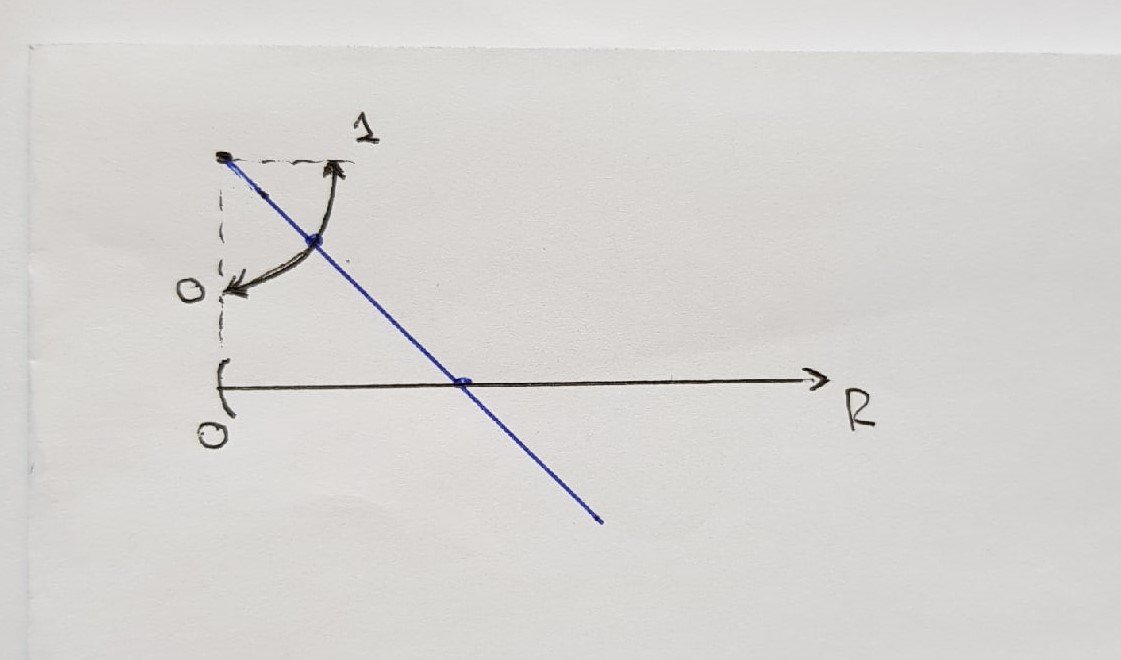
\includegraphics[width=0.7\textwidth]{p_a}
\end{center}
Интервал $(0, 1)$ биективен согнутной в дугу окружности этой же длины, которая образует четверть окружности. Любая прямая, проходящая через центр окружности и точку на дуге пересекает числовую прямую и этим отображение мы покроем всю прямую. Отображение взаимно однозначно, так как через любые 3 точки проходит лишь единственная прямая.
\item $[0, 1] \rightarrow [0, 1)$\\
Биекция задаётся следующим образом:
$$
\begin{aligned}
&f\left(\frac{1}{2}\right)=1\\
&f\left(\frac{1}{3}\right)=\frac{1}{2}\\
\end{aligned}
$$
\begin{center}
 $\ldots $
\end{center}
$$
\begin{aligned}
&f\left(\frac{1}{n+1}\right)=\frac{1}{n}
\end{aligned}
$$
Числа, которые не подчиняются этому уравнению переходят сами в себя (то есть $f(x) = x$)
\item $[0, 1] \rightarrow [0, 1]^2$\\
Для начала докажем, что отрезок $[0, 1]$ равномощен множеству бесконечных последовательностей нулей и единиц. Будем записывать число $x \in [0, 1]$ в виде бесконечной двоичной дроби (бесконечной двоичной последовательности):\\
Первый знак после запятой равен 0, если $x$ лежит в левой половине отрезка $[0, 1]$, и равен 1, если в правой. Чтобы определить следующий бит, нужно поделить выбранную половину снова пополам. Если $x$ лежит в левой половине, то следующая цифра 0, а если в правой, то 1. И так далее: чтобы определить очередной знак, нужно поделить текущий отрезок пополам и посмотреть, в какую половину попадает x.\\
Но после таких действий мы не получим взаимнооднозначного соответствия между числами на отрезке $[0, 1]$ и бесконечными двоичными последовательностями, так как нет взаимнооднозначности, когда $ x $ попадает на границу раздела (тогда можно выбрать как правую, так и левую половину и в итоге получим, что одному и тому же числу соответствует 2 бесконечные двоичные последовательности: например, $0,001111 \ldots$ и $0,01000 \ldots$ соответствуют одному и тому же числу) \\
Чтобы сделать взаимнооднозначное соответствие исключим последовательности, в которых начиная с некоторого момента все цифры равны 1 (кроме одной: $ 0,1111 \ldots $ - соответствует 1). Таких последовательностей счётное число и они не влияю на равномощность. Тогда получим биекцию.\\

Получили, что между отрезоком $[0, 1]$ и множеством бесконечных последовательностей нулей и единиц можно установить биекцию, значит, между квадратом $[0, 1]^2 $ и множеством упорядоченных пар таких последовательностей тоже можно установить биекцию (пара соответсвующая точки $ (x,y) $ соответсыует паре составленной из последовательностей $ x $ и $ y $)\\
Биекцию между бесконечными последовательностями нулей и единиц и парами таких последовательностей устанавливаем таким образом: паре последовательностей $ a_0,a_1,a_2 \ldots b_0,b_1,b_2 \ldots $ ставим в соответствие последовательность $ a_0,b_0,a_1,b_1,a_2,b_2 \ldots $ (обратное отображение: выделяем отдельно чётные и отдельно нечётные).

\item $2^\mathbb{N} \rightarrow [0, 1]$\\
Множество всех подмножеств множества натуральных чисел можно задать множеством бесконечных последовательностей нулей и единиц (1 -- берём элемент в множество, 0 -- не берём). А множество бесконечных последовательностей нулей и единиц биективно $[0, 1]$, как мы доказали в прошлом пункте.
\end{itemize}

\end{document} % конец документа